\documentclass{presis}

\usepackage{../custompkgs/commands}
\usepackage{../custompkgs/presistyle}
\usepackage{../custompkgs/presicolors}

\begin{document}
\maketitle

\begin{frame}{Structure}
\tableofcontents
\end{frame}

\section{The World of Positive Scalar Curvature}
\sectionframe{../img/psc_inv.png}

\begin{frame}{Scalar Curvature}
    \begin{defi}
Let $(M,g)$ be a Riemannian manifold of dimension $n$.
The scalar curvature of $g$ is the function $\scal_g\colon M\to \R$ that appears in the taylor expansion
\begin{equation*}
    \frac{\vol(B_r(x))}{\vol(B_r^{\text{euklid}})} = 1 - \frac{\scal_g(x)}{6(n+2)}r^2 + \dots
\end{equation*}
\end{defi}
\end{frame}

\begin{frame}{Examples}
    $$\frac{\vol(B_r(x))}{\vol(B_r^{\text{euklid}})} = 1 - \frac{\scal_g(x)}{6(n+2)}r^2 + \dots$$\pause
    \begin{vfilleditems}
    \item Any onedimensional Riemannian manifold has vanishing scalar curvature.\pause
    \item Euclidean space $(\R^n,g_{\text{euklid}})$ has vanishing scalar curvature.\pause
    \item The sphere $S^n\subset\R^{n+1}$ has constant positive scalar curvature when $n>1$.\pause
    %\item The torus $T^n = \R^n/\Z^n$ can be given a metric of scalar curvature zero.\pause
    \item The projective space $\RP^n$ can be given a metric of positive scalar curvature when $n>1$.
    \end{vfilleditems}
\end{frame}

\begin{frame}{More Examples}
    %In dimension $2$, scalar curvature of a surface $M$ is just twice the Gaussian curvature $K$.\pause
    Let $M\subset \R^3$ be an embedded surface.\pause
    The Gauss--Bonnet-theorem says 
    \begin{equation*}
        \int_M K \,\mathrm{d}A = 2\pi \:\chi(M)
    \end{equation*}\pause
    So the only embedded surface that admits a metric of positive scalar curvature is $S^2$.
\end{frame}

\begin{frame}{Properties}
    Let $(M,g)$ and $(M^\prime,g^\prime)$ be Riemannian manifolds, and $\lambda\in \R$ a constant.\pause 
    We then have
    \begin{vfilleditems}
        \item Scaling: $\scal_{\lambda g}(x) = \frac{1}{\lambda} \scal_g(x)$ for all $x\in M$.\pause
        \item Additivity: $\scal_{g\oplus g^\prime}(x,x^\prime) = \scal_g(x) + \scal_{g^\prime}(x^\prime)$ for any $(x,x^\prime)\in M\times M^\prime$.
    \end{vfilleditems}\pause
    Thus if $M$ admits a metric of positive scalar curvature, so does $M\times M^\prime$ for any closed $M^\prime$.
\end{frame}

\begin{frame}{Existence}
    A manifold $M$ is called \psc-manifold, if it admits a metric of positive scalar curvature.\pause
    \begin{thm}[Gromov--Lawson, Schoen--Yau, 1980]
    Let $M$ be a simply connected manifold of dimension $n \geq 5$. If $M$ is not spinnable, $M$ is a \psc-manifold.
    \end{thm}\pause
    $\rightarrow$ Spinnable case finished by Stolz in '92: vanishing of $\hat{\mathfrak{a}}(M)$ neccesary and sufficient.
\end{frame}


\begin{frame}{Generalization}
    Call $\mR^+(M)$ the space of \psc-metrics (with $C^\infty$-topology) on $M$.\pause
    \begin{thm}[Ebert--Wiemeler, 2022]
        Let $M$ be a simply connected spin manifold of dimension $n\geq 5$. Then
        \begin{equation*}
            \mR^+(M) \whe \mR^+(S^d)
        \end{equation*}
        whenever $M$ admits a \psc-metric.
    \end{thm}\pause
    $\rightarrow$ Simply connected, nonspinnable case similarly handled.
\end{frame}

\begin{frame}{Method}
    \begin{thm}[Ebert--Wiemeler, 2022]
        Let $M$ and $M^\prime$ be $n$-manifolds of tangential $2$-type $(B,\t)$ and $x\in \Omega_n^\t$ \good, such that $[M] \equiv [M^\prime] + x$ in $\Omega_n^\t$.
    Then if $n\geq 5$
    \begin{equation*}
        \mR^+(M) \whe \mR^+(M^\prime).
    \end{equation*}
    \end{thm}\pause
    $\rightarrow$ There are six tangential $2$-types. For each one, obtain a theorem.\\\pause
    $\rightarrow$ $\theta=\BSpin\to\BO$ gives the result on the previous slide
\end{frame}

\begin{frame}{Step-by-Step}
    Fix a dimension $n\geq5$. Let $W$ be an $n$-dimensional manifold of tangential $2$-type $(B,\t)$.\pause
    \begin{vfilleditems}
    \item[\protect\circled{1}] Compute a set of generators of $\Omega_n^\t$.\pause
    \item[\protect\circled{2}] Prove that all those generators are \good.{\only<6->{\color{warncolor}$\leftarrow$ What if they aren't?}}\pause
    \item[\protect\circled{3}] Obtain $\mR^+(M) \whe \mR^+(W)$ for any $M$ with tangential $2$-type $(B,\t)$.
        {\color{black} The subgroup of the good generators is the whole group, so this is a special case.} %hack so that line spacing fits the next slide.
    \end{vfilleditems}\pause
    $\rightarrow$ In other words, there is only one possible homotopy type of $\mR^+(M)$ for manifolds of this tangential $2$-type in dimension $n$.
\end{frame}

\begin{frame}{Step-by-Step\only<5->{ in our Case}}
    Fix a dimension $n\geq 5$. Let $W$ be an $n$-dimensional manifold of tangential $2$-type \only<-5>{$(B,\t)$}\only<6->{{\color{warncolor} $(\BO,\id_\BO)$}}.
    \begin{vfilleditems}
    \item[\protect\circled{1}] Compute a set of generators of \only<-6>{$\Omega_n^\t$}\only<7->{{\color{warncolor}$\NN_n$}}.\pause
    \item[\protect\circled{2}] Find a (hopefully large) subset of of \good{} generators.\pause
    \item[\protect\circled{3}] Obtain $\mR^+(M) \whe \mR^+(W)$ for any $M$ with tangential $2$-type \only<-7>{$(B,\t)$}\only<8->{{\color{warncolor} $(\BO,\id_\BO)$}} and $M \equiv W$ in \only<-7>{$\Omega_n^\t/_{\mathcal{A}_n}$}\only<8->{${\color{warncolor}\NN_n}/_{\mathcal{A}_n}$}, where $\mathcal{A}_n$ is the subgroup generated by the \good{} generators.\pause
    \end{vfilleditems}
    \only<5->{\color{\beamerbgcolor}}
    $\rightarrow$ Notice, that $\left\lvert\Omega_n^\t/_{\mathcal{A}_n}\right\rvert$ is an upper bound for the amount of different homotopy types of $\mR^+(M)$ in dimension $n$.
\end{frame}

\section{Calculations in the Unoriented Bordism Groups}
\sectionframe{../img/abord_inv.png}

\begin{frame}{Bordism}
    \begin{defi}
        Call two closed $n$-dimensional manifolds $M,M^\prime$ bordant, if there is a manifold $W$ of dimension $n+1$ with boundary $\partial W = M \amalg M^\prime$.
    \end{defi}\pause
    $\rightarrow$ Defines an equivalence relation on the set of all closed $n$-dimensional manifolds.\pause \\
    $\rightarrow$ The set of equivalence classes forms an abelian group $\NN_n$ with disjoint union $\amalg$ as sum.
\end{frame}

\begin{frame}{Ring Structure}
    \begin{defi}
        The (unoriented) bordism ring is the unital, commutative, graded ring
        \begin{equation*}
            \NN_\ast = \left(\bigcup\limits_{n\in\N} \NN_n, \amalg, \times, [\emptyset], [\{\ast\}]\right)
        \end{equation*}
    \end{defi}\pause
    $\rightarrow$ Surprisingly, $\NN_n$ is finite for each $n$.\pause \\
    $\rightarrow$ Furthermore, the entire ring is well understood...
\end{frame}

\begin{frame}{Thoms work}
    \begin{thm}[Thom--Dold, 1954-1956]
        The unoriented bordism ring is isomorphic to a polynomial algebra over $\zz$, with precicely one generator in each degree $n\neq 2^k - 1$.
        Generators are represented by Dold-manifolds $P(m,n)$.
    \end{thm}\pause
    $\rightarrow$ Define $P(m,n) = S^m\times\CP^n /_\sim$ where $(x,z)\sim (-x,\overline{z})$.\pause \\
    $\rightarrow$ Notice $P(m,0) \cong \RP^m$.
\end{frame}

\begin{frame}{Thoms work more precicely}
    \begin{vfilleditems}
    \item In even dimension $n = 2m$, we have a multiplicative generator given by $[P(2m,0)] = [\RP^{2m}]$.\pause
    \item In odd dimension $n = 2^r(2s + 1) - 1$, we have a multiplicative generator given by $[P(2^r - 1, s2^r)]$ whenever $n\neq 2^k - 1$.\pause
    \end{vfilleditems}
    $\rightarrow$ Additive generators of $\NN_n$ correspond to partitions of $n$ that contain no element of form $2^k - 1$.
\end{frame}

\begin{frame}{Additive Generators}
    An additive generator of $\NN_n$ has the general form
    \begin{equation*}
        \left[ \prod\limits_{i\in I} (\RP^{2i})^{m_i} \times \prod\limits_{j\in J} P(2^{r_j} - 1, s_j 2^{r_j}) \right]
    \end{equation*}
    where $\sum_{i\in I} (2 m_i i) + \sum_{j\in J} (2^{r_j}(2 s_j + 1) - 1) = n$.\\\vspace{\baselineskip}, and $I,J\subset\N$. \pause
    $\rightarrow$ Now: Which of those are \good ?
\end{frame}

\begin{frame}{Good Generators I}
\begin{lem}[Ebert--Wiemeler, 2022]
    Let $M \to M^\prime$ be a smooth fiber bundle with fiber $\KP^{n + m - 1}$. Then $[M]$ is \good{} if either ...
    \begin{itemize}
        \item $\K = \R$, $n,m\geq 3$ with structure group $O(m)\times O(n) / \{\pm 1\}$
        \item $\K = \C$, $n,m \geq 2$ with structure group $U(n)\times U(m)$.
        \item $\K = \C$, $n + m -1 \geq 3$ with structure group $\zz$.
        \item $\K = \HH$, $n,m\geq 1$ with structure group $\mathrm{Sp}(n)\times\mathrm{Sp(m)}/\{\pm 1\}$
    \end{itemize}
\end{lem}\pause
    $\rightarrow$ Remember Rokhlin's Trick: $[\RP^n\times\RP^n] = [\CP^n]$, $[\CP^n\times\CP^n] = [\HP^n]$.
\end{frame}

\begin{frame}{Good Generators II}
    Repeatedly applying the above yields, that all (additive) generators are \good{}, except maybe those of form 
    \begin{equation*}
        (\RP^2)^{i} \times (\RP^4)^{j} \times P(1,2)^k
    \end{equation*}
    where $i=0,1,2,3$ and $j=0,1$ as well as $k\in\N$.\pause{} 
    But theres more...\pause
    \begin{lem}[Ebert--Wiemeler]
        Elements of form $[M^\prime \times P(1,2)]$ are \good , if $M^\prime$ has a \psc-metric.
    \end{lem}
\end{frame}

\begin{frame}{Good Generators III}
    There are only finitely many generators left of which we dont know  whether they are \good.\pause{}
    \begin{align*}
        n = 2,\quad & \RP^2 & \only<3->{{\color{warncolor} \leftarrow \text{ Theorem doesn't apply}}}\\
        n = 4,\quad & \RP^4, \CP^2 & \only<3->{{\color{warncolor} \leftarrow \text{ Theorem doesn't apply}}}\\
        n = 6,\quad & \RP^2\times\CP^2, \RP^2\times\RP^4 & {\color{\beamerbgcolor} \leftarrow \text{ our Theorem does apply}} \\
        n = 8,\quad & \RP^4\times\CP^2 & \\
        n = 10,\quad & \RP^2\times\RP^4\times\CP^2 & 
    \end{align*}\pause\pause
    $\rightarrow$ In particular, for dimension $>10$ all additive generators are \good, and we obtain our theorem.
\end{frame}

% frame asking for questions
\begin{frame}[plain, noframenumbering]
    \centering
    \vfill
    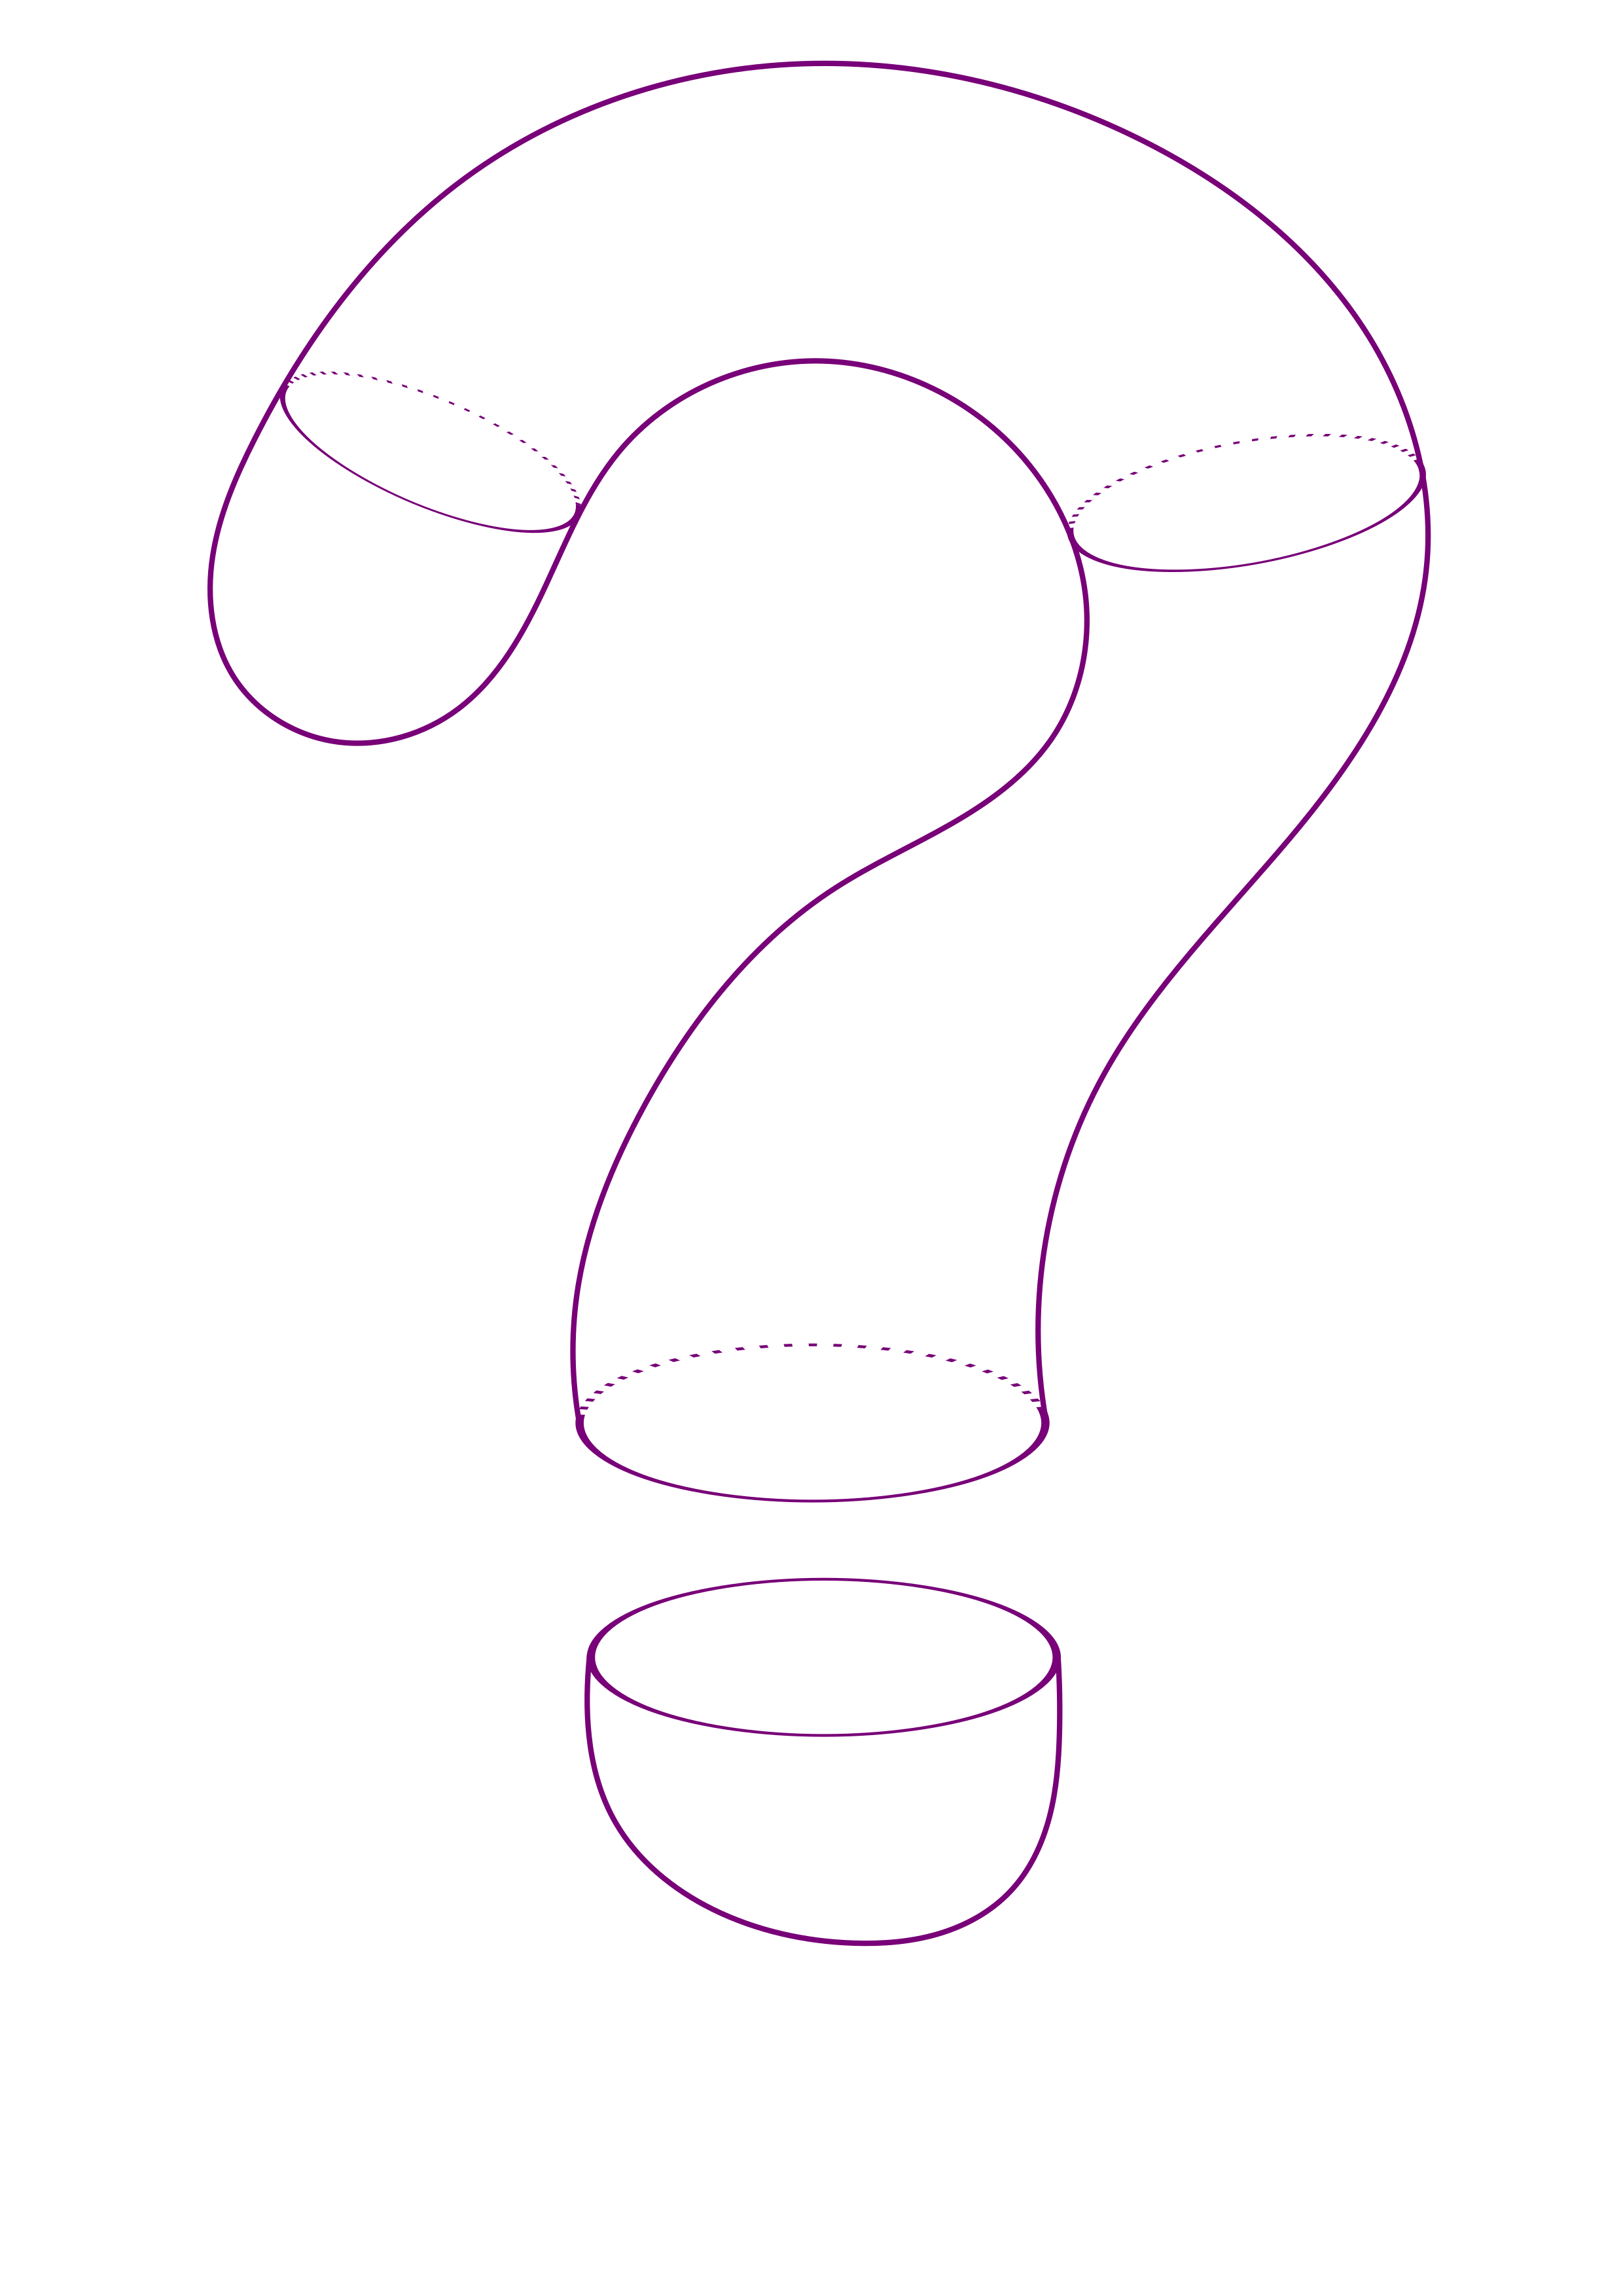
\includegraphics[width=.4\linewidth]{../img/questionmark.png}
    \vfill
\end{frame}

\begin{frame}{Main Result}
    \begin{thm}
    Let $M$ be a $n$-dimensional Manifold of tangential $2$-type $\id_\BO$, and $n>10$. Then
    \begin{equation*}
        \mR^+(M) \whe \mR^+(S^{n-6}\times\RP^2\times\CP^2)
    \end{equation*}
    \end{thm}\pause
    $\rightarrow$ The manifold $S^{n-6}\times\RP^2\times\CP^2$ is just an arbitrary reference manifold with the correct tangential $2$-type.
\end{frame}

\appendix % stops frame max numbering here
\section*{$\t$-Structures and Tangential $2$-Types}
\sectionframe{../img/moebius_inv.png}

\begin{frame}{$\t$-Structures}
    \begin{defi}
        Let $\t\colon B\to \BO$ be a fibration. 
        A $\t$-structure on a manifold $M$ is a lift of the stable tangent bundle $\st\colon M \to \BO$ along $\t$.
    \end{defi}\pause
    $\rightarrow$ Generalizes orientations via $\t\colon \BSO \to \BO.$\\\vspace{.3\baselineskip} \pause
    $\rightarrow$ Generalizes spin structures via $\t\colon\BSpin \to \BO$.\\\vspace{.3\baselineskip}\pause
    $\rightarrow$ Every manifold has a canonical $\id_\BO$-structure.
\end{frame}

\begin{frame}{Tangential Type}
    \begin{defi}
        A $\t$-structure on $M$ is called tangential $k$-type of $M$, if the $\t$ is $k$-coconnected and the lift is $k$-connected.
    \end{defi}\pause
    $\rightarrow$ Unique up to fiber homotopy equivalence.\\\vspace{.3\baselineskip}\pause
    $\rightarrow$ Tangential $1$-type is either $\BSO\to\BO$ or $\id_\BO$, depending on $w_1$.
\end{frame}

\begin{frame}{Tangential $2$-types}
\begin{thm}
    Let $G = \pi_1(M)$ and $w_i$ denote the Stiefel--Whitney-classes of $M$.
    Call $\widetilde{w}_2= w_2(\widetilde{M})$.
    Then the tangential $2$-type of $M$ is:
    \begin{itemize}
        \item $\BO \times_{\B \zz} \B G$, if $\widetilde{w}_2 \neq 0, w_1 \neq 0$
        \item $\BSO \times \B G$, if $\widetilde{w}_2 \neq 0, w_1 = 0$
        \item $\B(G,w_1,w_2)$, if $\widetilde{w}_2 = 0$.
    \end{itemize}
\end{thm}\pause
    $\rightarrow$ These are six cases, as $\widetilde{w}_2 \neq 0$ implies $w_2 \neq 0$.
\end{frame}

\end{document}
